\justifying
\begin{problem}{1}
	Ліхтар масою $m = 10$ кг висить посередені вулиці шириною $l = 10$ м. Допустима сила натягу канату $T = 500$ Н. На якій висоті $H$ можуть бути закріплені кінці канатц, щоб точка підвісу ліхтаря знаходиласт на висоті $h = 5$  м?
	
	\begin{figure}[h!]
		\begin{subfigure}{.4\textwidth}
			\centering
			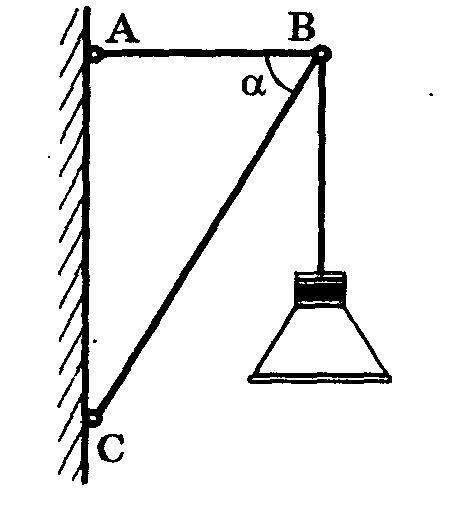
\includegraphics[width=0.5\linewidth]{class8/gelf_58}
			\caption{}
			\label{fig:gelf58}
		\end{subfigure}
		\begin{subfigure}{.4\textwidth}
			\centering
			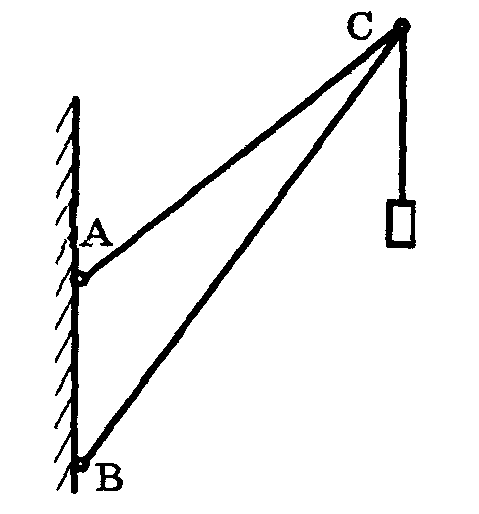
\includegraphics[width=0.5\linewidth]{class8/gelf_59}
			\caption{}
			\label{fig:gelf59}
		\end{subfigure}
		\begin{subfigure}{.4\textwidth}
			\centering
			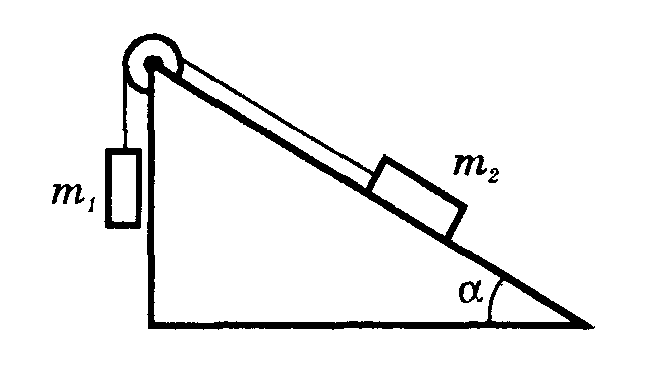
\includegraphics[width=0.5\linewidth]{class8/gelf_512}
			\caption{}
			\label{fig:gelf512}
		\end{subfigure}
	\end{figure}
\end{problem}


\begin{problem}{3}
	Невагомі стержні AB та BC шарнірно закріплені в точках А, В та С (рис.). Чому рівні сили, які діють на стержні, якщо $\alpha = 60^{\circ}$, а маса ліхтаря, який підвішено в точці В $m = 3$ кг?(див. рис. \ref{fig:gelf58})
\end{problem}



\begin{problem}{5}
	Вантаж масою $m_2$ знаходиться на похилій плозині, яка утворює кут $\alpha$ з горизонтом. Коефіцієнт тертя рівен $\mu$. На нитці, яка прив'язана до вантажу і перекинута через блок, підвішено вантаж $m_1$. При якій величині $m_1$ система буде знаходитись в рівновазі? (див. рис. \ref{fig:gelf512})
	
\end{problem}

\begin{problem}{6}
	До стержня довжиною $l = 120$ см та масою $m = 8$ кг підвішено два вантажки: до лівого кінця -- вагою $P = 30$ Н, а до правого -- вагою $P = 90$ Н. Стержень підвісили на одній нитці так, що він знаходиться в рівновазі. На якій відстані від лівого кінця стержня знаходиться точка рівноваги?
\end{problem}




\textbf{Задачі для самостійного розв'язання}

\begin{problem}{2}
	З якою силою $F$ необхідно тягнути за мотузку, яка прив'язана до ящика масою $m = 40$ кг і яка утворює кут $\alpha = 30^{\circ}$ з горизонтом, щоб ящик рухався горизонтальною поверхнею рівномірно?
\end{problem}

\begin{problem}{4}
	Знайти сили, які діють на шарнірно закріплені стержні $BC$ та $AC$, якщо $AB = 60$ см, $AC = 1.2$ м, $BC = 1.6$ м. Маса вантажу $50$ кг (див. рис. \ref{fig:gelf59})
\end{problem}

\begin{problem}{7}
	До балки масою $m_1 = 400$ кг та довжииною $l = 7$ м підвішено вантаж масою $m_2 = 700$ кг на відстані $a = 2$ м від одного з його кінців. Балка своїми кінцями лежить на опорах. Яка сила тиску на кожну з цих опор?
\end{problem}